\documentclass[10pt]{article}
\usepackage{ucs}
\usepackage[a4paper, total={6in, 10in}]{geometry}
\usepackage[utf8x]{inputenc}
\usepackage{graphicx}
\title{Essential Skills: Assignment Computer architecture}
\date{2 October 2016}
\author{Ali Abdulmadzhidov}

\begin{document}
\renewcommand*\rmdefault{cmss}
\maketitle
\section{Digital circuit}
We add 1000 (right to left) from constant's. Output on leds is 1001. \\ \\
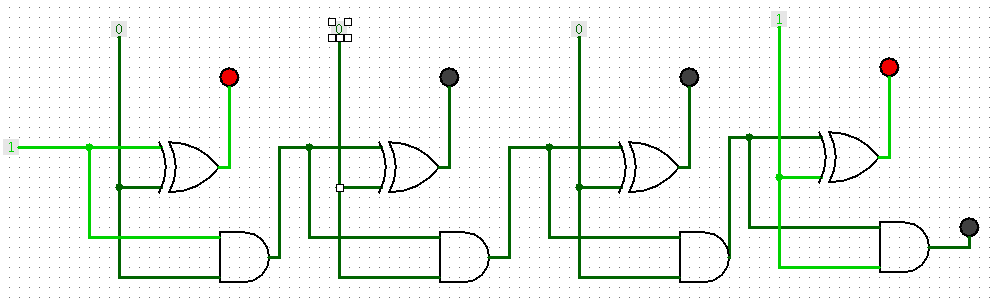
\includegraphics[width=\textwidth, scale=0.5]{circuit1} \\ \\
We add 1010 (right to left) from constant's. Output on leds is 1011 \\ \\
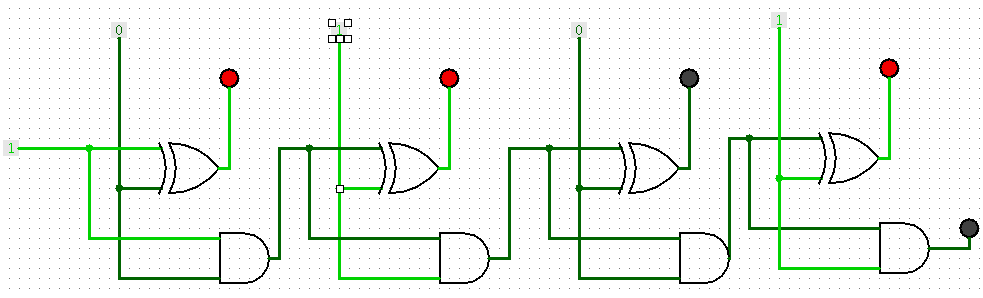
\includegraphics[width=\textwidth, scale=0.5]{circuit2} \\ \\

Same with 6 elements \\ \\
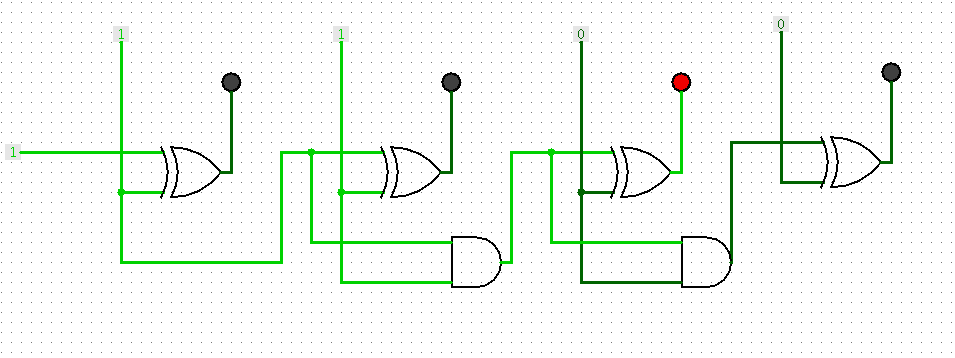
\includegraphics[width=\textwidth, scale=0.5]{circuit3} \\ \\

\section{Perfomance measurement}
\subsection{Installation SIM-PL}
\begin{enumerate}
    \item Downloading SimPL and components
        \begin{verbatim}
            wget https://staff.fnwi.uva.nl/t.r.walstra/innopolis/SIM-­PL_2.3.0.zip
            wget https://staff.fnwi.uva.nl/e.h.steffens/Downloads/Arco/Innopolis/ComponentLab1.zip
        \end{verbatim}
    \item Unzipping
        \begin{verbatim}
            unzip SIM-­PL_2.3.0.zip -d SIMPL
            unzip components_lab_1.zip -d comps
        \end{verbatim}
    \item Executing executor
        \begin{verbatim}
            cd SIMPL
            java -jar executor.jar
        \end{verbatim}
    \item File-Open needed architecture. Than in code viewer file-open needed asm program. 
\end{enumerate}

\subsection{Measuring parameters.}
    \subsubsection{Singlecycle. Assume that we have 10hz clock rate}
        \subsubsection{ForLoop.asm}
        \begin{enumerate}
            \item 45 instructions
            \item CPI - 1
            \item CpuTime = 4.5sec. 
        \end{enumerate}
        \subsubsection{Addition.asm}
        \begin{enumerate}
            \item 6 instructions
            \item CPI - 1
            \item CpuTime = 0.6sec
        \end{enumerate}
        \subsubsection{Square.asm}
        \begin{enumerate}
            \item 99 instructions
            \item CPI - 1
            \item CpuTime = 9.9sec  
        \end{enumerate}

    \subsubsection{Multicycle. Assume that we have 50hz clock rate}
        \subsubsection{ForLoop.asm}
        \begin{enumerate}
            \item 46 instructions
            \item CPI - 3.8
            \item CpuTime = 3 sec 
        \end{enumerate}
        \subsubsection{Addition.asm}
        \begin{enumerate}
            \item 6 instructions
            \item CPI - 3.6
            \item CpuTime = 0.44 sec
        \end{enumerate}
        \subsubsection{Square.asm}
        \begin{enumerate}
            \item 117 instructions
            \item CPI - 3.5
            \item CpuTime = 7.08 sec
        \end{enumerate}

    \subsubsection{Pipelined Assume that we have 50hz clock rate}
        \subsubsection{ForLoop.asm}
        \begin{enumerate}
            \item 25 instructions
            \item CPI - 1
            \item CpuTime = 0.5 seс
        \end{enumerate}
        \subsubsection{Addition.asm}
        \begin{enumerate}
            \item 108 instructions
            \item CPI - 1
            \item CpuTime = 2.16 sec
        \end{enumerate}
        \subsubsection{Square.asm}
        \begin{enumerate}
            \item 128 instructions
            \item CPI - 1
            \item CpuTime - 2.56 sec            
        \end{enumerate}


\subsection{Explain the following}
    \begin{enumerate}
        \item addition.asm was performed good by three archs. In forloop and square pipelined was the best, cause it can it has shorter cycle and can divide instrcutions to execute them in one time.
        \item program counter shows memory adress of instruction that is executing now or'll be executed next
        \item multicycle take more then one cycle to execute instruction.
        \end{enumerate}
\subsection{Explain the following}
    \begin{enumerate}
        \item ADDI - adds a register and a sign-extended immediate value and saves result in another register
        \item NOP - command that does nothing. Used to make delay or to force memory alignment.
        \item LI - puts number to register.
        \begin{verbatim}li $s0, 123 # puts 123 to #s0\end{verbatim}
        \item BNE - jumps to label
        \begin{verbatim}
        label:  li $s0, 0
                BNE label
        \end{verbatim}
    \end{enumerate}

\subsection{Subtracting 2 variables}
\begin{verbatim}
    # Generated assembly code
    @include "Mips.wasm"
     
    #
    .data MyRegisters : REGISTERS
    0x00 : WORD 0x00 # put $0 to zero (default assumption)
     
    .data MyMemory : DATAMEM
    0x00 : WORD 0x00
     
    # De instructiecodes worden in
    .code MyCode: MIPS, MyMemory
     
    # Sla getal 1 op in register 1
    LI      $4, 1
    ADD     $1, $4, $0
     
    # Sla getal 2 op in register 2
    LI      $5, 2
    ADD     $2, $5, $0
     
    # Tel register 1 en 2 bij elkaar op
    # en plaats het resultaat in register 3
    SUB     $6, $1, $2
    ADD     $3, $6, $0
     
    # - Orginal C code -
    #{
    #       int a;
    #       int b;
    #
    #       int result;
    #
    #       a = 1;
    #       b = 2;
    #
    #       result = a - b;
    #
    #}

\end{verbatim}

\end{document}